\chapter{Grundlagen}
\section{Physikalische Grundlagen} 
\subsection{Peltier-Element}
\section{Elektrotechnische Grundlagen}
\subsection{Buck-Converter}
Im folgendem soll die Funktion eines Buck-Converter vereinfacht wiedergegeben.


\section{Regelungsstechnische Grundlagen}
\subsection{z-Transformation}
Um Übertragungsfunktionen digital berechnen zu können muss eine z-Transformation durchgeführt werden. Die z-Transformation ähnelt der Laplacetransformation für kontinuerliche Signale, wobei die z-Transformation auf Zahlenfolgen angewendet wird.
\begin{equation}
f^*(t) = \sum_{k=0}^\infty f(kT)\delta(t-kT)
\end{equation}
Über den Dirackkamm mit der Periodendauer T, wird die kontinurliche funktion abgetastet. Sie ist nur zu den Abtastzeitpunkten $t=kT$ von null verschieden. Wendet man die Laplace Transformation auf die Zahlenfolge an folgt
\begin{equation}
F^*(s) = \mathcal{L}(f^*(t)) = \sum_{k=0}^\infty f(kT)e^{-ksT}
\end{equation}
Für $e^{sT}$ führt man nun die komplexe Variabel z ein
\begin{equation}
z = e^{sT}
\end{equation}
Damit ergibt sich
\begin{equation}
F^*(s) = \mathcal{L}(f^*(t)) = \sum_{k=0}^\infty f(kT)z^{-k}
\end{equation}
Für eine beliebige Folge
\begin{equation}
f(k) = (f(0), f(1), f(2), ...)
\end{equation}
erhält man so die z-Transformierte zu
\begin{equation}
F(z) = f(0) + f(1)z^{-1} + f(2)z^{-2} + ...
\end{equation}
Es ist ersichtlich das $z^{-1}$ gleichbedeuteten mit einer Zeitverschiebung um die Abtastzeit ist. Gesucht wird im folgenen eine Aproximation um aus dem Laplacebereich in den z-Bereich zu gelangen. Wenn die Exponentialreihe 
\begin{equation}
z = e^{sT} = 1+sT+\frac{1}{2}(sT)^2 + ...
\end{equation}
nach dem zweiten Glied abbgebrochen wird folgt daraus
\begin{equation}
s\, \Laplace  \, \frac{z-1}{T}
\end{equation}
Es sei erwähnt das dies nur eine Nährung der z-Transformierten ist. Es existiert eine exakte Transformation die aber mehr theoretische Einfühurung benötigt. Die Güte der Approximation ist von der Abtastzeit $T$ und der Steilheit der Funktion abhängig. In der vorliegenden Arbeit soll die Approximation verwendet werden.
\cite[vgl.][S.501ff.]{Lunze2014}

\subsection{PT1-Strecke}
Ein Verzögerungsglied 1. Ordnung, das einen Integratoren und damit einen Energiespeicher besitzt, wird $PT_2$-Strecke genannt. Sie ist für die Modellierung vieler physikalischer Strecken oder für Filteranwendungen geeignet. Der Wirkplan zeigt den Aufbau der Strecke.
\begin{figure}[H]
\makebox[\textwidth]{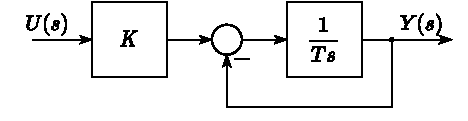
\includegraphics[width=\linewidth-20mm]{kapitel2/images/PT1Struktur}}
\caption{PT1-Struktur}
\label{Grundlagen:PT1Struktur}
\end{figure}
Die Übertragungsfunktion ergibt sich aus der Struktur \ref{Grundlagen:PT1Struktur} zu
\begin{equation}
G(s) = K\frac{T}{s+T}
\end{equation}
Mit der statischen Verstärung $K$ und der Zeitkonstante $T$. Die Sprungantwort im Zeitbereich ergibt sich zu
\begin{equation}
h(t) = k(1-e^{-\frac{t}{T}})
\end{equation}
Bei $t=T$ ergibt sich daraus
\begin{equation}
h(T) = k(1-e^{-1}) \approx 0.63
\end{equation}
Diese Eigenschaft kann für die Parametrierung von PT1-Strecken verwendet werden. Um die Strecke als digitalen Filter zu verwenden muss die Übertragungsfunktion diskretisiert werden. Im folgenem soll über eine Aproximation durch den Rückwärts-Differenzenquotient das System Diskretisiert werden. Für LTI Systeme kann über die Transformation von dem Bildbereich in den Z-Bereich eine exakte Diskretisierung vorgenommen werden. Diese benötigt mehr Therorie und ist nicht so intuitiv wie die Approximation.
\cite[vgl.][S.501ff.]{Lunze2010}



